\chapter{\textsc{Analyse du procédé de deux bacs d'eau sans entrée}}
\section{\textsc{Le procédé}}
 
 \paragraph{} Le système représenté sur la Figure 2 est composé de deux bacs cylindriques de section $S$. Ils sont reliés par
un tuyau de section $S_n << S$, où l’eau peut circuler dans les deux directions. Lors de cette manipulation, nous
allons nous intéresser au niveau de l’eau $H_1 (t)$ et $H_2 (t)$.

\paragraph{} Les valeurs données par le constructeur sont : $ S = 0.0154m^2 $ et $S_n = 5 \times 10^{-5}m^2 $. Les valeurs initiales sont $ H_1 (0) = 0.3m $ et $ H_2 (0) = 0.2m $.

	\begin{center}
	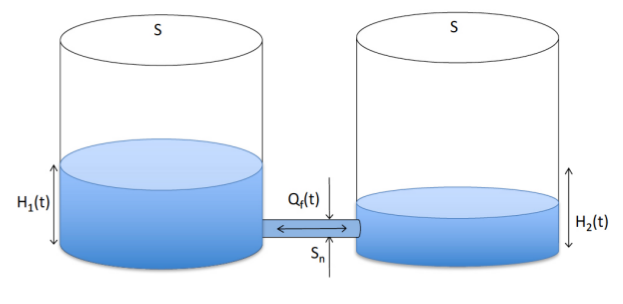
\includegraphics[scale=0.5]{2bac.png}
	\captionof{figure}{\textit{Deux bacs d'eau sans source et fuite\\}}
	\label{fig2} 
	\end{center}
	
\section{\textsc{Modélisation du système par un bilan de volume}}

	Nous avons:
\begin{center}
    $$\left\{
\begin{array}{l}
    V(t)=S\times H(t)\\
    \dot{V}(t)=S\times \dot{H}(t)=(Q(t)-Q_f(t)) ;\text{ avec Q(t) = $0$.}\\
    Q_f(t)=S_n \times V_n \ ; \ \ \ avec\indent  V^2_n = 2\times g\times |H_1(t)-H_2(t)| 

\end{array}
\right.$$
\end{center}


Donc $Q_f(t)=S_n\sqrt{2g |H_1(t)-H_2(t)|}$\\\\
On pose:  $ x= H_1 - H_2$

\[\Longrightarrow Q_f=S_n\times \sqrt{2\times g \times |x|}\]
\[\Longrightarrow \dot{x}=-\frac{Q_f}{S}=-sign(x)\times \frac{S_n\times \sqrt{2\times g }}{S} \times \sqrt{|x|}\]
\[\color{red}\dot{x}=-sign(x)\times \frac{S_n\times \sqrt{2\times g }}{S} \times \sqrt{|x|}\]
 Avec: \textbf{sign(x)} représente le sens de l'écoulement de l'eau entre les deux bacs. \\
 
\textbf{Hypothèse:} on suppose que $H_1>H_2$.\\
\\
Alors:\indent \indent  \[\dot{x}= -\frac{S_n\times \sqrt{2\times g }}{S} \times \sqrt{x}\]
\\
\\
\\\\\\\\

\section{Détermination du point d'équilibre}

On cherche \textbf{x} tel que \textbf{x}= Cst = $\textbf{X}_0$

\[0=-\frac{S_n\times \sqrt{2\times g }}{S} \times \sqrt{X_0}\indent  \Longrightarrow \indent X_0 = 0\]
Cela signifie que le niveau de l'eau dans les deux bacs est le même $H_1=H_2$.

\section{Linéarisation autour du point d'équilibre:}

\[\dot{\delta_x}=f(X_0+\delta_x) \indent \Longrightarrow \indent \dot{\delta_x}=f(X_0)+\frac{\partial f}{\partial x}(X_0).\delta(x)\]
Sachant que $f(X_0)=0$ ;\indent  $\Longrightarrow \indent \dot{\delta_x}=\frac{\partial f}{\partial x}_{|X_0} . \delta_x$
\[\dot{\delta_x}=\begin{bmatrix}\frac{-S_n\times \sqrt{2\times g}}{2\times S \times \sqrt{X0}}\end{bmatrix}.\delta_x \ \ ; \indent \longleftarrow \indent \text{Or, ceci est impossible}\]
Donc, la linéarisation est impossible.

\section{Simulation du modèle non-linéaire:}


\begin{figure}[H]
    \centering
    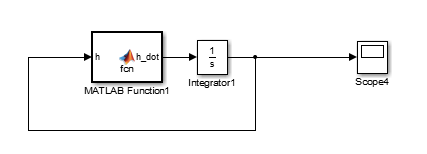
\includegraphics[width=\textwidth]{part2.PNG}
    \caption{Schéma Simulink}
    \label{fig:part2}
\end{figure}

On simule pour une condition initiale $X=0.1= H_1-H_2$\\
Le système autonome converge vers le point d'équilibre $H_1=H_2$ donc vers $X_0=0$


\begin{figure}[H]
    \centering
    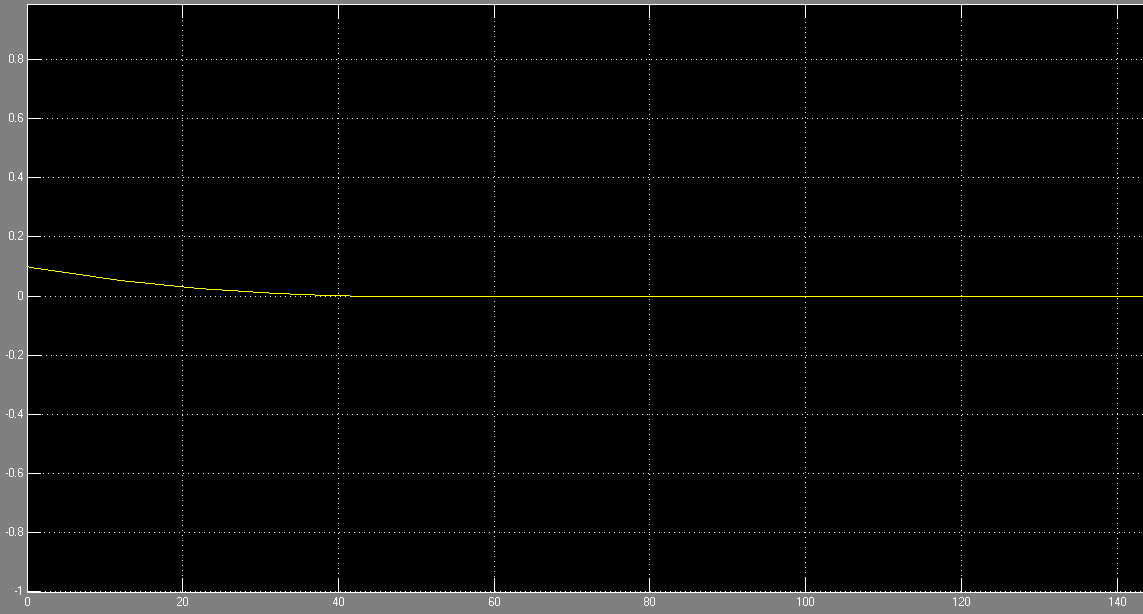
\includegraphics[width=\textwidth]{autonom.PNG}
    \caption{Résultats du modèle non-linéare }
    \label{fig:autonom}
\end{figure}

	
	
\section{\textsc{Fonction de Lyapunov pour le modèle non-linéaire}}

	\par On choisira la même fonction utilisée précédemment soit :$ V(x) \frac{x^2}{2} $, sa dérivée devient:
	 
	\begin{center}
	
		$ \dot{V} (x) = \frac{-S_n}{S} \sqrt{2gx} \hspace{1mm} x  \hspace {0.5 cm} $ si $H_1(t) > H_2(t) $	
	 
	\end{center}
	\par Sachant que $x=H_1(t) - H_2(t)$ alors $x>0$ or la quantité $\frac{-S_n}{S} \sqrt{2gx}<0$, cela prouve que $\dot{V}(x)$ est définie négative pour $H_1(t) > H_2(t)$, le deuxième cas présente:  
	
	\begin{center}
	
		$ \dot{V} (x) = \frac{S_n}{S} \sqrt{2gx}\hspace{1mm} x \hspace{0.5 cm}$ si $H_1(t) < H_2(t) $
			
	\end{center}
	
	\par Sachant que dans ce cas $x<0$ et la quantité $\frac{S_n}{S} \sqrt{2gx}>0$ alors $V(x)$ est définie négative si $H_1(t) < H_2(t)$
	\par De cette façon la fonction dérivée de Lyapunov est définie négative pour les deux cas, donc le système est globalement asymptotiquement stable. 
	 